% !TeX spellcheck = en_US
\documentclass[french]{yLectureNote}

\title{Introduction à la thermodynamique}
\subtitle{Thermodynamique}
\author{Paulhenry Saux}
\date{\today}
\yLanguage{Français}

\professor{}

\usepackage{graphicx}%-pour mettre des images
\usepackage[utf8]{inputenc}%encodage
\usepackage{geometry}%pour modifier les tailles et mettre a4paper
%\usepackage{awesomebox}%pour les boites d'exercices, de pbq et de croquis d\'esactiv\'e pour les TP de PC
\usepackage{tikz}%pour deiffner + d\'ependance de chemfig
\usepackage{tkz-tab}
\usepackage{tabularx}%pour dimensionner automatiquement les tableaux avec variable X
\usepackage{awesomebox}%Pour les boites info, danger et autres
\usepackage{menukeys}%Pour deiffner les touches de Calculatrice
\usepackage{fancyhdr}%pour les en-t\^ete personnalis\'ees
\usepackage{blindtext}%pour les liens
\usepackage{hyperref}%pour les liens (\`a mettre en dernier)
\usepackage{caption}%pour la francisation de la l\'egende table vers Tableau
\usepackage{pifont}
\usepackage{array}%pour les tableaux
\usepackage{lipsum}
\usepackage{yFlatTable}
\usepackage{multicol}
\newcommand{\Lim}[1]{\lim\limits_{\substack{#1}}\:}
\renewcommand{\vec}{\overrightarrow}
\newcommand{\bz}{\overline{z}}
\DeclareMathOperator{\card}{card}
\renewcommand{\vec}{\overrightarrow}
\newcommand{\N}[0]{\mathbb{N}}
\newcommand{\R}[0]{\mathbb{R}}
\newcommand{\C}[0]{\mathbb{C}}
\newcommand{\dd}[0]{\mathrm{d}}
\newcommand{\er}{\vec{e_{\rho}}}
\newcommand{\ep}{\vec{e_{\varphi}}}
\newcommand{\pip}{\pi^+}
\newcommand{\pim}{\pi^-}
\newcommand{\mv}{\mathcal{V}}
\DeclareMathOperator{\Div}{Div}
\newcommand{\rot}{\vec{\mathrm{rot}}}
\newcommand{\grad}{\vec{\mathrm{grad}}}
\begin{document}
\setcounter{chapter}{7}
\chapter{Machines thermiques}
\section{Introduction}
\begin{itemize}
    \item Tous les résultats seront par unité de masse.
    \item Certains états physiques sont assimilés à des états d'équilibre.
    \item Les échanges de chaleur sont imaginés avec des sources.
    \item C'est cyclique : on revient à l'état initial
\end{itemize}
Il faut souvent imaginer la dernière transformation, ce qui est une différence importante avec les processus réels.
\section{Résultats généraux}
\subsection{cycle monotherme}
On applique le premier principe : $\Delta U_{cycle} = W_{cycle}+Q_{c} = 0\Rightarrow W = -Q$

Le deuxième principe : $S_{cycle}^P = \Delta S_C-S^e = -\frac{Q}{T_S}>0\Rightarrow Q_s <0$

Donc $W>0$ : on ne peut que récupérer du travail pour le transformer en chaleur.


\subsection{cycle ditherme}
On applique le premier principe : $W_c + Q_F+Q_C = 0$

$S_C^p = -\frac{Q_F}{T_F}- \frac{Q_c}{T_c}$

Donc si $W = 0 , Q_c=-Q_f$ et si $ S_p = 0, Q_c = -\frac{T_c}{T_f}Q_f$.

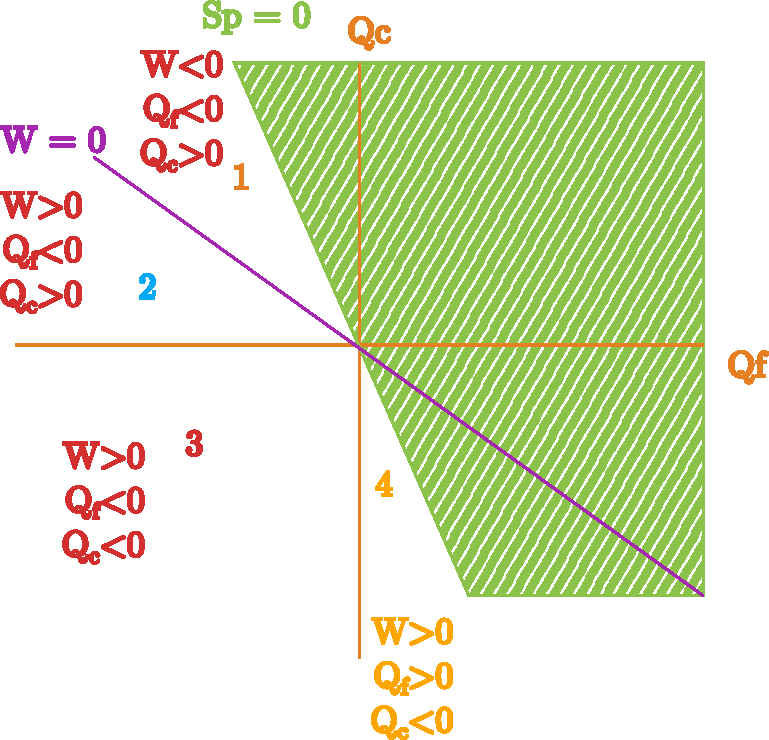
\includegraphics[scale=0.5]{graphe}

On va donc étudier 2 machines dithermes :

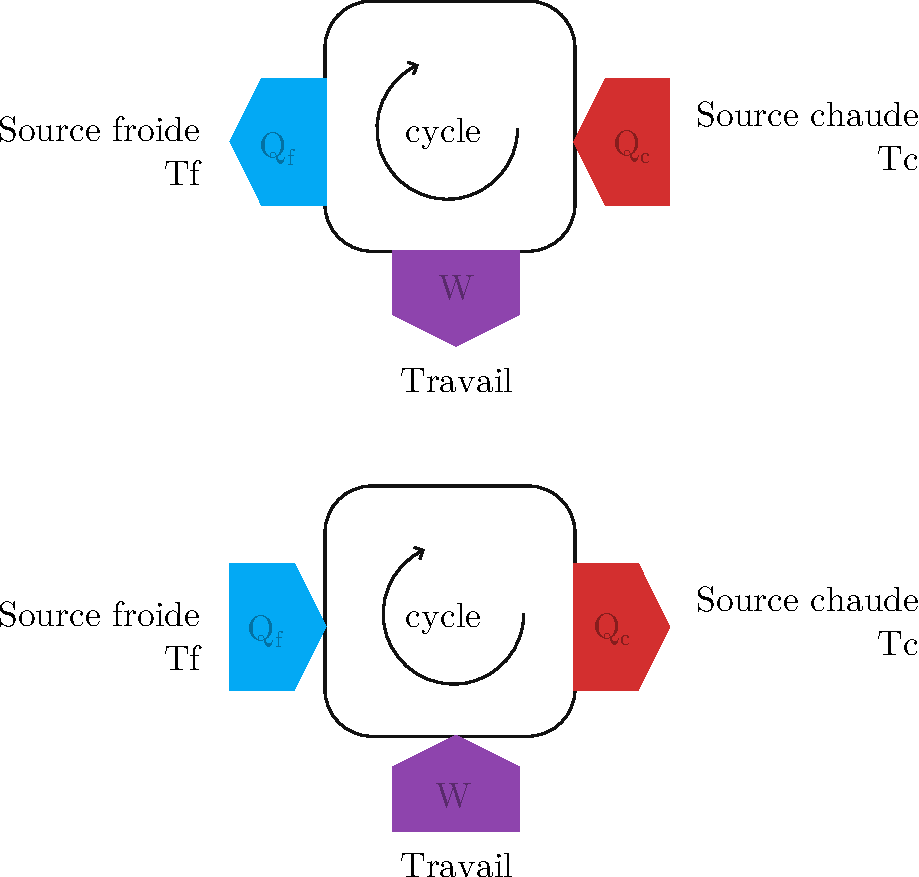
\includegraphics[scale=0.5]{2machines.pdf}

\subsection{Efficacité des machines thermiques dithermes}
\begin{definition}[Efficacité énergétiques]
    $\eta_{PAC} = |\frac{Q_c}{W}|$

    $\eta_{Frigo} = |\frac{Q_f}{W}|$

    $\eta_{Moteur} = |\frac{W}{Q_c}|$
\end{definition}
Pour des cycles réversibles, on a 
\begin{theorem}[Valeur d'efficacité max]
    $\eta_{max} = 1 -\frac{T_f}{T_c}$. Cette valeur est atteinte lors de cycle réversible. C'est l'efficacité de Carnot
\end{theorem}
Avec 2 sources, le seul cycle réversible possible est le cycle de Carnot.

%TODO Démonstration du cycle de Carnot
Plus on veut une température de source froide faible, plus il faut engager de l'énergie (= du travail).
\section{Cycles spécifiques}
\subsection{Cycles de Lenoir,  Beau et Rochas et Diesel}
\subsubsection{Cycle de Lenoir}
\begin{itemize}
    \item $A\to B$ : échauffement isochore au contact de $S_c$
    \item $B\to D$ : Détente adiabatique + QS = Phase motrice
    \item $D\to A$ : refroidissement monobare ay contact de $S_f$
\end{itemize}
On cherche à déterminer
\begin{itemize}
    \item $Q_c = Q_{AB} = \Delta U_{AB} = mc_v(T_B-T_A) = mc_v(T_{sc}-T_{sf})$
    \item $Q_f =  \Delta H_{DA} = mc_v(T_A-T_D) = mc_v(T_{sf}-T_{D})$ :
    \item $W$ :
\end{itemize}
on veut exprimer $T_D$ en fonction des données : $T_BV_B^{\gamma-1} = T_DV_D^{\gamma-1}$. On en déduit que 
$T_D = T_{D} = T_{sc}(\frac{V_A}{V_D})$

On pose $\alpha = \frac{T_{sf}}{T_{sc}}$ et $\beta = \frac{V_{max}}{V_{min}}$

De plus, $p_b/p_a = T_sc/T_sc$ et $p_b/p_a = \beta^\gamma$

On en déduit que $Q_F = mc_p(T_{sf}-T_{sc}\alpha^{\frac{\gamma-1}{\gamma}})$

On en déduit le travail puis l'efficacité.
$\eta_M = 1+ \gamma \frac{\alpha-\alpha^{(\gamma-1)/\gamma}}{1-\alpha}$
%détailler le calcul en TODO
RMQ : Puissance motrice : $P_w = |\frac{W}{Z_{cycle}}|$
\subsubsection{Cycle de beau et rochas = modèle du moteur à explosion}
%TODO moteur 2
On veut trouver 
\begin{itemize}
    \item $Q_c = \Delta U_{BD} = mc_v(T_D-T_B)$
    \item $Q_F = \Delta U_{DE} = mc_v(T_A-T_E)$
    \item 
\end{itemize}
On pose $\beta = \frac{V_{max}}{V_{min}}$

On obtient : $\eta = 1- \frac{(\frac{1}{\beta})^{\gamma-1}T_Sc-T_SF}{T_SC-T_SF\beta^{\gamma-1}}$
\subsection{Cycle de Rankine et Hirn}
%TODO Cycle de rankine
\end{document}


